\chapter{Network Bending: Direct and Expressive Manipulation of Generative Neural Networks}
\label{ch:net_bend}

\section{Introduction}

This chapter details the work I undertook in developing the Network Bending framework, a way to directly manipulate the internet features of generative models during inference. This work was first published online as a pre-print on arxiv \citep{broad2020network}, then later a revised manuscript was accepted as a conference paper at EvoMUSART \citep{broad2021network}, and then as an extended journal paper in Entropy \citep{broad2022network}.
The experiments in the original paper were done for the task of image generation with StyleGAN2. 
A follow up study applying the same techniques to a custom VAE trained on spectrograms was later done for the extended Entropy paper. 
In this chapter, they are written chronologically.

\section{Motivation}

\section{Transformation Layers}

% \begin{figure}[!htbp]
%     \centering
%     \includegraphics[width=1\textwidth]{images/NB/Transform-Figure.png}
%     \caption[A comparison of various network bending transforms applied to various layers in StyleGAN2.]{A comparison of various transformation layers inserted and applied to all of the features in different layers in the StyleGAN2 network trained on the FFHQ dataset, showing how applying the same filters in different layers can make wide-ranging changes the generated output. The rotation transformation is applied by an angle $\theta=45$. The scale transformation is applied by a factor of $k_{x}=k_{y}=0.6$. The binary threshold transformation is applied with a threshold of $t=0.5$. The dilation transformation is applied with a structuring element with radius $r=2$ pixels.}
%     \label{fig:layerwide_comparison}
% \end{figure}

I implemented a broad variety of deterministically controlled transformation layers that can be dynamically inserted into the computational graph of the generative model. 
The transformation layers are implemented natively in PyTorch \citep{paszke2019pytorch} for speed and efficiency. I
 treated the activation maps of each feature of the generative model as 1-channel images in the range -1 to 1. 
 Each transformation is applied to the activation maps individually before they are passed to the next layer of the network. 

 The transformation layers can be applied to all the features in a layer, or a random selection, or by using pre-defined groups automatically determined based on spatial similarity of the activation maps (Section \ref{section:clustering}). 
 Figure \ref{fig:layerwide_comparison} shows a comparison of a selection of these transformations applied to all the features layer-wide in various layers of StyleGAN2.

\subsection{Numerical Transformations}

I began with simple numerical transformations $f(x)$ that are applied to individual activation units $x$. 
I implemented four distinct numerical transformations: the first is \emph{ablation}, which can be interpreted as $f(x) = x \cdot 0$. 
The second is \emph{inversion}, which is implemented as $f(x) = 1 - x$. 
The third is \emph{multiplication by a scalar} $p$ implemented as $f(x) = x \cdot p$. 
The final transformation is \emph{binary thresholding} (often referred to  as posterisation) with threshold $t$, such that:
\begin{equation}
f(x) = \begin{cases}
    1,& \text{if } x\geq t\\
    0,              & \text{otherwise}
\end{cases}
\end{equation}

\subsection{Affine Transformations}
\label{sec:affine}
For this set of transformations, each activation map $X$ for feature $f$ is treated as an individual matrix that simple affine transformations can be applied too. 
The first two are horizonal and vertical \emph{reflections} that are defined as:
\begin{equation}
X \begin{bmatrix}
-1 & 0 & 0\\
\ 0 & 1 & 0\\
\ 0 & 0 & 1
\end{bmatrix}\quad , \quad X \begin{bmatrix}
1 & \ 0 & 0\\
0 & -1 & 0\\
0 & \ 0 & 1
\end{bmatrix}
\end{equation}

\noindent The second is \emph{translations} by parameters $p_x$ and $p_y$ such that:
\begin{equation}
X \begin{bmatrix}
1 & 0 & p_x\\
0 & 1 & p_y\\
0 & 0 & 1
\end{bmatrix}
\end{equation}

\noindent The third is \emph{scaling} by parameters $k_x$ and $k_y$ such that:
\begin{equation}
X \begin{bmatrix}
k_x & 0 & 0\\
0 & k_y & 0\\
0 & 0 & 1
\end{bmatrix}
\end{equation}
Note that in this chapter, I only report on using uniform scalings, such that $k_x = k_y$. Finally, fourth is \emph{rotation} by an angle $\theta$ such that:
\begin{equation}
X \begin{bmatrix}
cos(\theta) & -sin(\theta) & 0\\
sin(\theta) & cos(\theta) & 0\\
0 & 0 & 1
\end{bmatrix}
\end{equation}

Other affine transformations can easily be implemented by designing the matrices accordingly.

\subsection{Morphological Transformations}

I implemented two of the possible basic mathematical morphological transformation layers, performing \emph{erosion} and \emph{dilation} \citep{soille1999erosion} when applied to the activation maps, which can be interpreted as 1-channel images. 
These can be configured with the parameter $r$ which is the radius for a circular kernel (aka structural element) used in the morphological transformations.

\textbf{FIGURE: morph transformation}

\section{Clustering Features}
\label{section:clustering}

As most of the layers in the current state of the art generative models, such as StyleGAN2, have very large numbers of convolutional features, controlling each one individually would be far too complicated to build a user interface around and to control these in a meaningful way. 
In addition, because of the redundancy existing in these models, manipulating individual features does not normally produce any kind of meaningful outcome. 
Therefore, it is necessary to find some way of grouping them into more manageable ensembles of sets of features. 
Ideally, such sets of features would correspond to the generation of distinct, semantically meaningful aspects of the image, and manipulating each set would correspond to the manipulation of specific semantic properties in the resulting generated sample. 
To achieve this, I developed a novel approach that combines metric learning and a clustering algorithm to group sets of features in each layer based on the spatial similarity of their activation maps. 
I trained a separate convolutional neural network (CNN) for each layer of the respective generative models (the StyleGAN2 generator and the decoder of our VAE) with a bottleneck architecture (first introduced by Gr{\'e}zl et al.~\citep{grezl2007probabilistic}) to learn a highly compressed feature representation; the later is then used in a metric learning approach in combination with the $k$-means clustering algorithm \citep{lloyd1982least, celebi2013comparative} to group sets of features in an unsupervised fashion. 

\subsection{Architecture}

For each layer of both generative models, I trained a separate CNN on the activation maps of all the convolutional features. 
As the resolution of the activation maps and number of features varies for the different layers of the model (a breakdown of which can be seen in Table \ref{tab:classifier-table}).
I employed an architecture that can dynamically be changed, by increasing the number of convolutional blocks, depending on what depth is required. 

\begin{table}[]
\centering
\begin{tabular}{|c|c|c|c|c|c|}%{llllll}
\hline
Layer & Resolution & \#features &  CNN depth & \#clusters & Batch size\\
\hline
1     & 8x8        & 512          & 1                & 5                & 500        \\
2     & 8x8        & 512          & 1                & 5                & 500        \\
3     & 16x16      & 512          & 2                & 5                & 500        \\
4     & 16x16      & 512          & 2                & 5                & 500        \\
5     & 32x32      & 512          & 3                & 5                & 500        \\
6     & 32x32      & 512          & 3                & 5                & 500        \\
7     & 64x64      & 512          & 4                & 5                & 200        \\
8     & 64x64      & 512          & 4                & 5                & 200         \\
9     & 128x128    & 256          & 5                & 4                & 80         \\
10    & 128x128    & 256          & 5                & 4                & 80         \\
11    & 256x256    & 128          & 6                & 4                & 50         \\
12    & 256x256    & 128          & 6                & 4                & 50         \\
13    & 512x512    & 64           & 7                & 3                & 20         \\
14    & 512x512    & 64           & 7                & 3                & 20         \\
15    & 1024x1024  & 32           & 8                & 3                & 10         \\
16    & 1024x1024  & 32           & 8                & 3                & 10       \\
\hline
\end{tabular}
\medskip
\caption[Table detailing model architecture for the ShuffleNet models used for clustering in StyleGAN2.]{
    \label{tab:classifier-table}Table showing resolution, number of features of each layer, the number of ShuffleNet \citep{zhang2018shufflenet} convolutional blocks for each CNN model used for metric learning, the number of clusters calculated for each layer using $k$-means and the batch size used for training the CNN classifiers for the StyleGAN2 models. Note: LSUN church and cat models have only 12 layers.
%\citep{lloyd1982least, celebi2013comparative}.
}
\end{table}

I employed the ShuffleNet architecture \citep{zhang2018shufflenet} for the convolutional blocks in the network, which is one of the state-of-the-art architectures for efficient inference (in terms of memory and speed) in computer vision applications. 
For each convolutional block, I utilised a feature depth of 50 and have one residual block per layer. 
The motivating factor in many of the decisions made for the architecture design was not focused on achieving the best accuracy per se. 
Instead, I wanted a network that can learn a sufficiently good metric while also being reasonably quick to train (with 12-16 separate classifiers required to be trained per StyleGAN2 model). 
I also wanted a lightweight enough network, such that it could be used in a real-time setting where clusters can quickly be calculated for an individual latent encoding, or it could be used efficiently when processing large batches of samples.

After the convolutional blocks, I flattened the final layer and learn from it a mapping into a narrow bottleneck $\vec{v} \in \mathbb{R}^{10}$, before re-expanding the dimensionality of the final layer to the number of convolutional features present in the layer of the respective generative model. 
The goal of this bottleneck is to force the network to learn a highly compressed representation of the different convolutional features in the generative model. 
While this invariably loses some information, most likely negatively affecting classification performance during training, this is in fact the desired result. 
I wanted to force the CNN to combine features of the activation maps with similar spatial characteristics so that they can easily be grouped by the clustering algorithm. 
Another motivating factor is that the chosen clustering algorithm ($k$-means) does not scale well for feature spaces with high dimensionality.

\subsection{Training}

I generated a training set of the activations of every feature for every layer of 1000 randomly sampled images and a test set of 100 samples for the models trained on all of the datasets used in our experiments. 
I trained each CNN using the softmax feature learning approach \citep{dosovitskiy2014discriminative}, a reliable method for distance metric learning. This method employs the standard softmax training regime \citep{bridle1990probabilistic} for CNN classifiers. 
Each classifier has been initialised with random weights and then trained for 100 epochs using the Adam optimiser \citep{kingma2015adam} with a learning rate of 0.0001 and with $\beta_1 = 0.9$ and $\beta_2 = 0.999$. 
All experiments were carried out on a single NVIDIA GTX 1080ti. The batch size used for training the classifiers for the various layers of StyleGAN2 can be seen in Table \ref{tab:classifier-table}. 
% The classifiers for the VAE were all trained with a batch size of 100.

After training, the softmax layer is discarded and the embedding of the bottleneck layer is used as the discriminative feature vector where the distances between points in feature space permit gauging the degree of similarity of two samples. 
This approach differs from standard softmax feature learning as it uses the feature vector from the bottleneck, rather than the last layer prior to softmax classification, giving a more compressed feature representation than the standard softmax feature learning approach.

\subsection{Clustering Algorithm}

Once each of the CNNs for every layer have been trained, they can then be used to extract feature representations of the activation maps of the different convolutional features corresponding to each layer of the generative model.
There are two approaches to this. The first is to perform the clustering on-the-fly for a specific latent for one sample. A user would want to do this to get customised control of a specific sample, such as a latent that has been found to produce the closest possible reproduction of a specific person from the StyleGAN2 model trained on the FFHQ dataset \citep{abdal2019image2stylegan,karras2019analyzing}. 
The second approach is to perform clustering based on an average of features' embedding drawn from many random samples, which can be used to find a general-purpose set of clusters.

The clustering algorithm for a single example is activated by a forward pass of the generative model performed without any additional transformation layers being inserted, to obtain the unmodified activation maps. 
The activation map $X_{df}$ for each layer $d$ and feature $f$ is fed into the CNN metric learning model for that layer $C_d$ to get the feature vector $\vec{v}_{df}$. 
The feature vectors for each layer are then aggregated and fed to the $k$-means clustering algorithm --- using Lloyd's method \citep{lloyd1982least} with Forgy initialization \citep{forgy1965cluster, celebi2013comparative}. 
This results in a pre-defined number of clusters for each layer. 
Sets of features for each layer can then be manipulated in tandem by the user.

Alternatively, to find a general purpose set of clusters, I first calculated the mean feature vector $\vec{\bar{v}}_{df}$ that describes the spatial activation map for each convolutional feature in each layer of generative model from a set of $N$ randomly generated samples --- the results in the paper are from processing 1000 samples. 
Then I performed the same clustering algorithm as previously for individual samples on the mean feature vectors. 
The number of clusters for each layer in StyleGAN2 can be seen in Table \ref{tab:classifier-table}.
%  Table \ref{tab:decoder-table} shows the number of clusters for each layer of the decoder of the spectrogram VAE.

\section{Manipulation Pipeline}

Transforms are specified in YAML (YAML Ain't Markup Language) configuration files \citep{ben2009yaml}, such that each transform is specified with 5 items: (i) the layer, (ii) the transform itself, (iii) the transform parameters, (iv) the layer type (i.e. how the features are selected in the layer: across all features in a layer, to pre-defined clusters, or to a random selection of features), and (v) the parameter associated with the layer type (either the cluster index, or the percentage of features the filter will randomly be applied to). 
There can be any number of transforms defined in such a configuration file.

After loading the configuration, the software either looks up which features are in the cluster index, or randomly apply indices based on the random threshold parameter. 
Then the latent is loaded, which can either be randomly generated, or be predefined in latent space $z$, or be calculated using a projection in latent space $w$ \citep{abdal2019image2stylegan,karras2019analyzing} (in the case of StyleGAN2). The latent code is provided to the generator network and inference is performed. 
As our implementation is using PyTorch \citep{paszke2019pytorch}, a dynamic neural network library, these transformation layers can therefore be inserted dynamically during inference as and when they are required, and applied only to the specified features as defined by the configuration. 
Once inference is unrolled, the generated output is returned. Figure \ref{fig:overview_diagram} provides a visual overview of the pipeline, as well as a comparison between a modified and unmodified generated sample.

\section{Results}

Talk about Clustering Results. Mainly from first paper etc.

\section{Network Bending in the Audio Domain}

\section{Discussion}


In this section, I discuss five perspectives: expressive manipulation, active divergence, comparisons of our results between the image and audio domains, comparisons with other methods, and finally show some real world examples where network bending has been used in the production of artworks.

\subsection{Expressive Manipulation}

The main motivation of the clustering algorithm presented in this chapter was to simplify the parameter space in a way that allows for more meaningful and controllable manipulations whilst also enhancing the expressive possibilities afforded by interacting with the system. 
These results show that the clustering algorithm is capable of discovering groups of features that correspond to the generation of different semantic aspects of the results, which can then be manipulated in tandem. 
These semantic properties are discovered in an unsupervised fashion and are discovered across the entire hierarchy of features present in the generative model. 
For example, Figure \ref{fig:cluster_layer_comp} shows the manipulation of groups of features across a broad range of layers that control the generation of: the entire face, the spatial formation of facial features, the eyes, the nose, textures, facial highlights and overall image contrast. Figure \ref{fig:cluster_audio_comp} shows our clustering algorithm performed in the audio domain, to demonstrate how aspects of the audio signal such as the transients and frequency components can be manipulated with various kinds of transformations.

% \begin{figure}[!htbp]
% \noindent \begin{centering}
%    \includegraphics[width=.2\textwidth]{images/NB/cluster_comparison/not_manipulated.png}
%    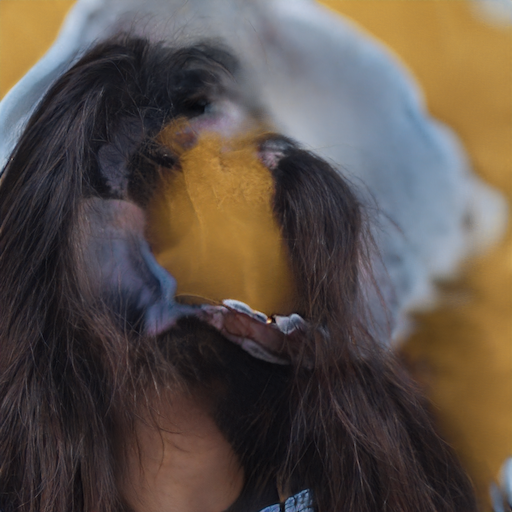
\includegraphics[width=.2\textwidth]{images/NB/cluster_comparison/layer_1_cluster0_mult-1.png}
%    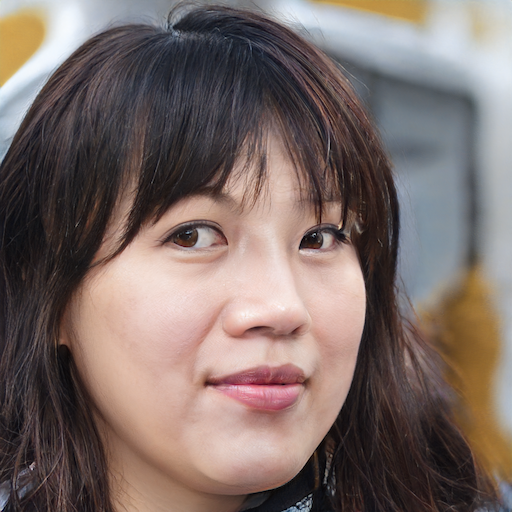
\includegraphics[width=.2\textwidth]{images/NB/cluster_comparison/layer_3_cluster2_mult5.png}
%    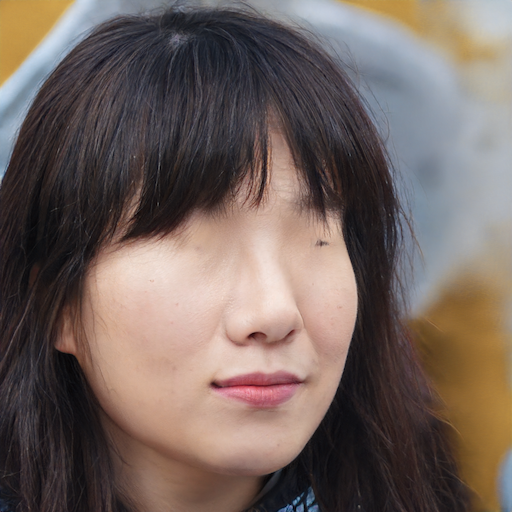
\includegraphics[width=.2\textwidth]{images/NB/cluster_comparison/layer_5_cluster2_ablate.png}
%    \par\end{centering}
%    \noindent \begin{centering}
%    \hfill (a)\hfill (b) \hfill (c) \hfill (d) \hfill\ %
%    \par\end{centering}
%    \smallskip
% \noindent \begin{centering}
%    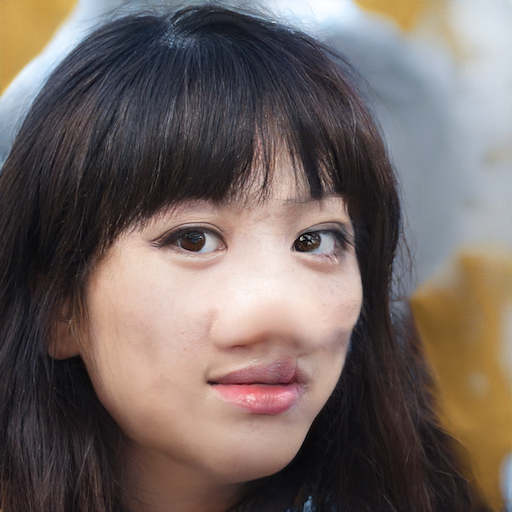
\includegraphics[width=.2\textwidth]{images/NB/cluster_comparison/layer_6_cluster4_dilate.png}
%    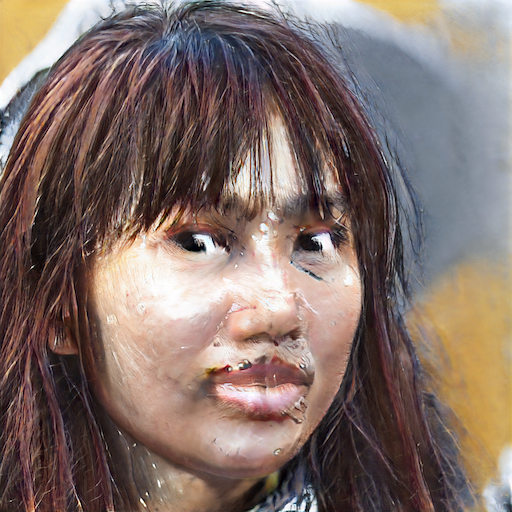
\includegraphics[width=.2\textwidth]{images/NB/cluster_comparison/layer_9_cluster3_mult5.png}
%    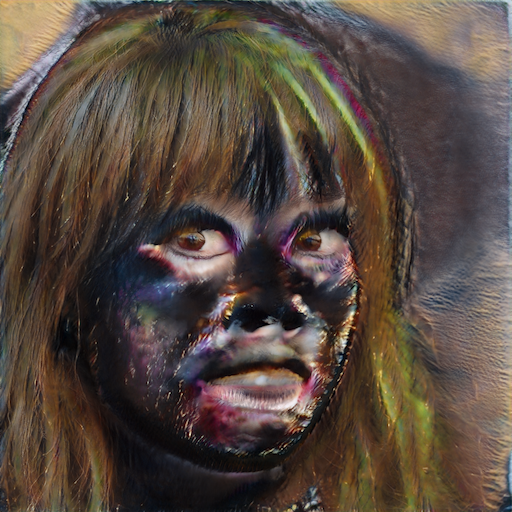
\includegraphics[width=.2\textwidth]{images/NB/cluster_comparison/layer_10_cluster0_mult-1.png}
%    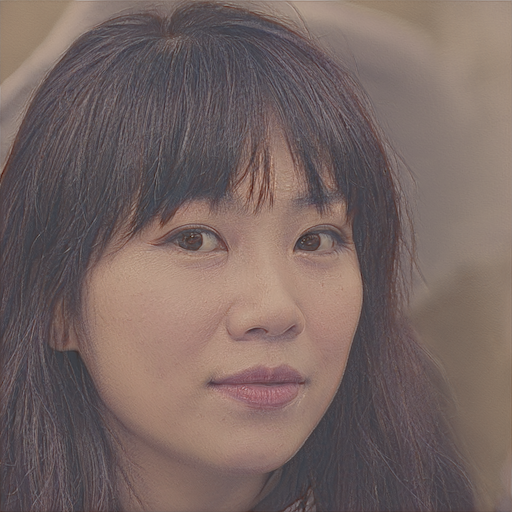
\includegraphics[width=.2\textwidth]{images/NB/cluster_comparison/layer_15_cluster0_mult0.1.png}
%    \par\end{centering}
%    \noindent \begin{centering}
%    \hfill (e)\hfill (f) \hfill (g) \hfill (h) \hfill\ %
%    \par\end{centering}
%    \caption[A comparison of different transforms being applied to different clusters in various layers of StyleGAN2.]{Examples from our clustering approach in the image domain. Clusters  of features in different layers of the model are responsible for the formation of different image attributes. (a) The unmanipulated result. (b) A cluster in layer 1 has been multiplied by a factor of -1 to completely remove the facial features. (c) A cluster in layer 3 has been multiplied by a factor of 5 to deform the spatial formation of the face. (d) A cluster in layer 6 has been ablated to remove the eyes. (e) A cluster in layer 6 has been dilated with a structuring element with radius $r=2$ pixels to enlarge the nose. (f) A cluster in layer 9 has been multiplied by a factor of 5 to distort the formation of textures and edges. (g) A cluster of features in layer 10 has been multiplied by a factor of -1 to invert the highlights on facial regions. (h) A cluster of features in layer 15 has been multiplied by a factor of 0.1 to desaturate the image. All transformations have been applied to sets of features discovered using our feature clustering algorithm (\S\ref{section:clustering}) in the StyleGAN2 model trained on the FFHQ dataset.}
%    \label{fig:cluster_layer_comp}
% \end{figure}


% \begin{figure}[!htbp]
% \noindent \begin{centering}
%    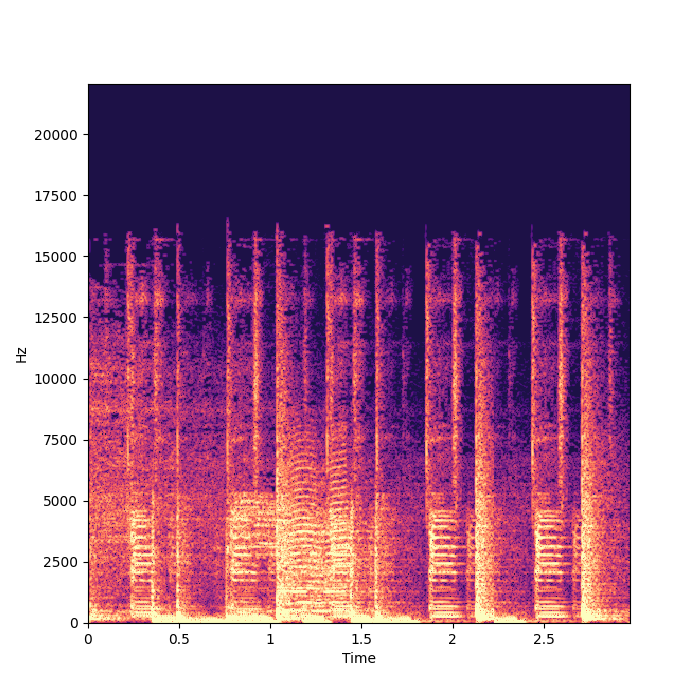
\includegraphics[width=.35\textwidth]{images/NB/audio_clusters/soul_short_original.png}
%    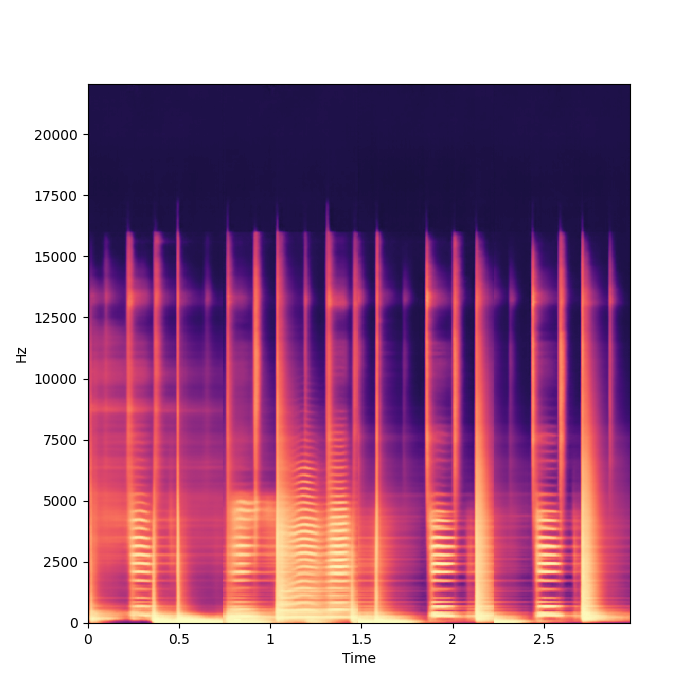
\includegraphics[width=.35\textwidth]{images/NB/audio_clusters/soul_short_reconstruction.png}
%    \par\end{centering}
%    \noindent \begin{centering}
%    \hfill (a)\hfill (b) \hfill \ %
%    \par\end{centering}
%    \smallskip
% \noindent \begin{centering}
%    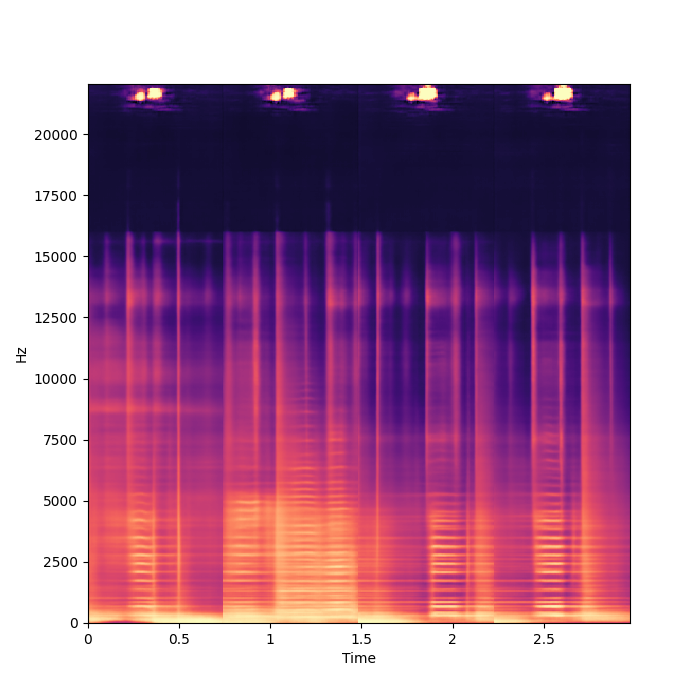
\includegraphics[width=.35\textwidth]{images/NB/audio_clusters/layer_1_cluster3_ablate.png}
%    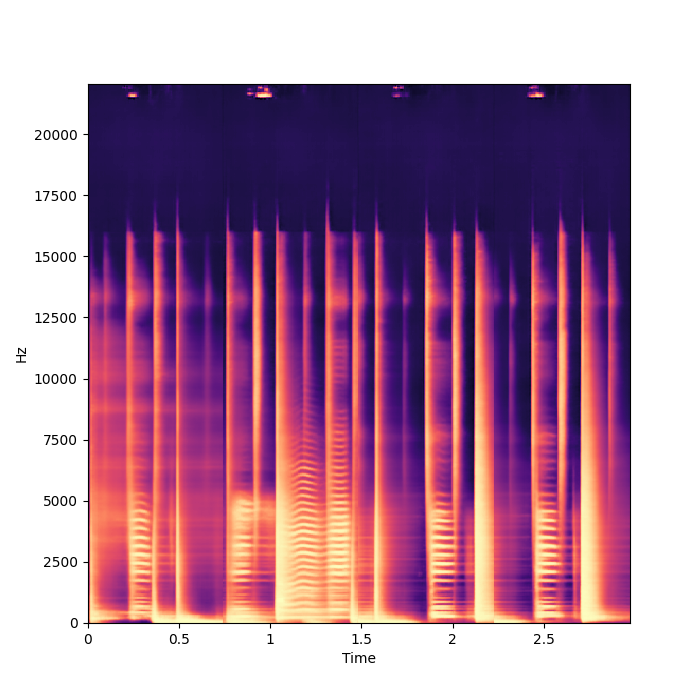
\includegraphics[width=.35\textwidth]{images/NB/audio_clusters/layer_1_cluster3_mult_2.png}
%    \par\end{centering}
%    \noindent \begin{centering}
%    \hfill (c)\hfill (d) \hfill \ %
%    \par\end{centering}
%    \smallskip
% \noindent \begin{centering}
%    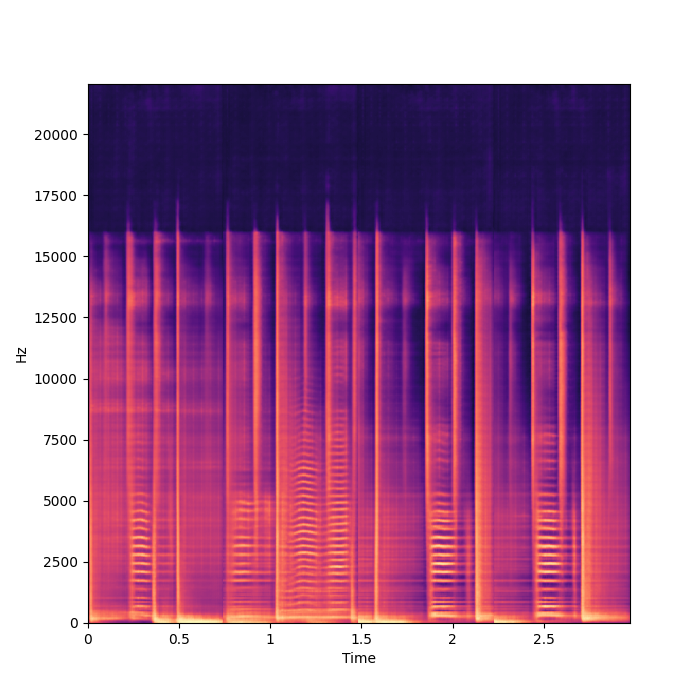
\includegraphics[width=.35\textwidth]{images/NB/audio_clusters/layer_3_cluster2_erode.png}
%    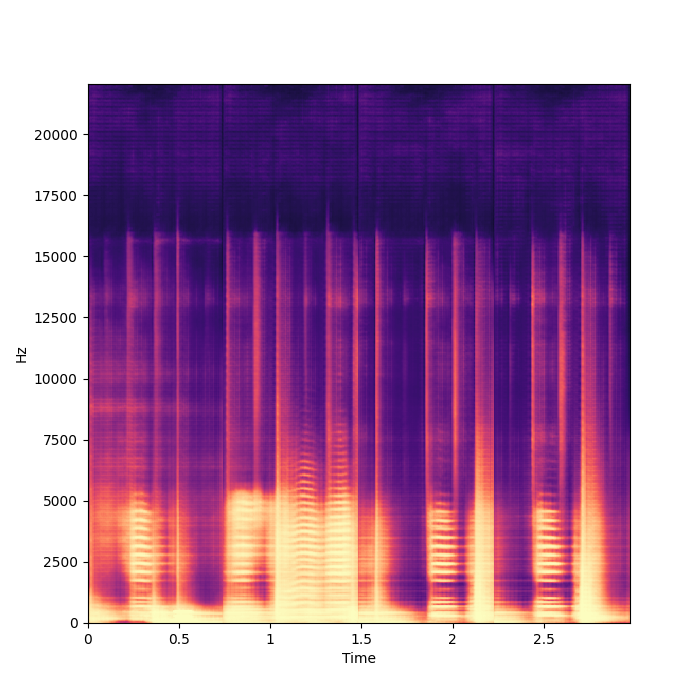
\includegraphics[width=.35\textwidth]{images/NB/audio_clusters/layer_3_cluster2_dilate.png}
%    \par\end{centering}
%    \noindent \begin{centering}
%    \hfill (e)\hfill (f) \hfill \ %
%    \par\end{centering}
%    \caption[A comparison of different transforms being applied to different clusters in various layers of the SpectrogramVAE.]{Examples from our clustering approach in the audio domain. (a) Spectrogram of an original source track not in the training set. (b) reconstruction of source track using VAE without manipulation. (c) Reconstruction of the same signal where a cluster in layer 1 responsible for the generation of the transients of the signal has been ablated. (d) Reconstruction of the same signal where the same cluster in layer 1 responsible for the transients has been multiplied by a factor of 2, increasing the intensity of the transients in the resulting signal. (e) Reconstruction of the signal where a cluster in layer 3 responsible for the low and mid-range frequencies has been eroded with a structuring element with radius $r=2$ pixels, diminishing the intensity of these frequency components. (f) Reconstruction of the signal where the same cluster in layer 3 responsible for the low and mid-range frequencies has been dilated with a structuring element with radius $r=2$ pixels, increasing the intensity of these frequency components. The audio sample used is a clip from \textit{Saulsalita Soul} by Mr.RuiZ, reproduced and transformed with permission granted under the CC BY-NC 4.0 licence.}
%    \label{fig:cluster_audio_comp}
% \end{figure}

Grouping and manipulating features in a semantically meaningful fashion is an important component of allowing expressive manipulation. 
However, artists are often also ready to consider surprising, unexpected results, to allow for the creation of new aesthetic styles, which can become uniquely associated with an individual or group of creators. 
Therefore the tool needs to allow for unpredictable as well as predictable possibilities, which can be used in an exploratory fashion and can be mastered through dedicated and prolonged use \citep{dobrian2006nime}. 
There is usually a balance between utility and expressiveness of a system \citep{jacobs2017supporting}. 
While it will be required to build an interface and perform user studies to more conclusively state that our approach has struck such a balance, our current results do show that both predictable semantic manipulation and more unpredictable, expressive outcomes are possible. 
This is a good indication that our approach represents a good initial step, and with further refinements, it can become an innovative powerful tool for producing expressive outcomes when using deep generative models. 

\subsection{Comparison Between Audio and Image Domains}

In this chapter I have demonstrated the network bending framework in both the image and audio domains. 
For the image domain, I have used StyleGAN2 \citep{karras2019analyzing}, the state of the art generative model for unconditional image generation, in the audio domain I have built our own custom generative model to demonstrate how the same principles of clustering features and applying transformations to clustered features can be applied indirectly to another domain. 
The generative model for audio I have presented is building on a much smaller body of research and has more room for improvement in terms of the fidelity of the generated outputs, however, it is still adequate and demonstrates that our clustering algorithm is capable of discovering semantically meaningful components of the signal (Figure \ref{fig:cluster_audio_comp}). 
Some of the transformation layers that were designed for image-based models such as rotation and scaling do not transfer meaningfully into the audio domain. 
However, numerical and morphological transformations do work effectively in the audio domain, representing a completely new approach for manipulating audio signals. 

\subsection{Comparison with Other Methods}

With respect to the semantic analysis and manipulation of a generative model, our approach of clustering features and using a broad array of transformation layers is a significant advance over previous works \citep{Bau2017-vg,Bau2018-td,bau2019semantic, Brink2019-gc}. 
This recent thread of techniques only interrogate the function of individual features, and as such are unlikely to be capable of capturing a full account of how a deep network generates results since such networks tend to be robust to the transformation of individual features. 

The results in this chapter show that sets of features, which may not be particularly responsive to certain transformations, are very responsive to others. 
Figure \ref{fig:ablation_comp} shows that in the model trained on the LSUN church dataset, a cluster of features, that when ablated has little noticeable effect on the result, can produce significant changes when using another transformation on the same cluster, here removing the trees and revealing the church building that was obscured by the foliage in the original result. 
This, I argue, shows that the functionality of features, or sets of features, cannot be understood only through ablation (which is the approach used in GAN dissection \citep{Bau2018-td}), because of the high levels of redundancy present in the learned network parameters. 
This shows that their functionality can be better understood by applying a wide range of deterministic transformations, of which different transformations are better suited to revealing the utility of different sets of features (Figures \ref{fig:cluster_layer_comp} \& \ref{fig:ablation_comp}).

% \begin{figure}[!htbp]
%    \centering
%    \subfloat{\includegraphics[width=.25\textwidth]{images/NB/church_ablation_comparison/not_manipulated.png}}
%    \subfloat{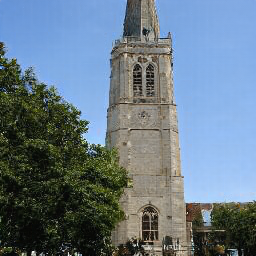
\includegraphics[width=.25\textwidth]{images/NB/church_ablation_comparison/layer_3_cluster1_ablate.png}}
%    \subfloat{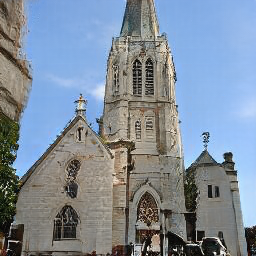
\includegraphics[width=.25\textwidth]{images/NB/church_ablation_comparison/layer_3_cluster1_mult5.png}}
%    \caption[A comparison of one cluster in StyleGAN2 having two different transforms applied to it.]{Groups of features that are not particularly sensitive to ablation may be more sensitive to other kinds of transformation. Left: original unmodified input. Middle: a cluster of features in layer 3 that has been ablated. Right: the same cluster of features that has been multiplied by a scalar of 5. As can be seen, ablation had a negligible effect, only removing a small roof structure that was behind the foliage. On the other hand, multiplying by a factor of 5 removes the trees whilst altering the building structure to have gable roof sections on both the left and right sides of the church - which are now more prominent and take precedence in the generative process. Samples are taken from the StyleGAN2 model trained on the LSUN church dataset.}
%    \label{fig:ablation_comp}
% \end{figure}

This method of analysis is completely \emph{unsupervised}, and does not rely on auxiliary models trained on large labelled datasets (such as in \citep{Bau2018-td, isola2017image, park2019semantic}) or other kinds of domain-specific knowledge. 
This approach therefore can be applied to any CNN based generative model architecture which has been trained on any dataset, as I have demonstrated by using the exact same clustering method for both image and audio domains. 
This is of particular relevance to artists who create their own datasets and would want to apply these techniques to models they have trained on their own data. 
Labelled datasets are prohibitively time consuming (and expensive) to produce for all but a few individuals or organisations. 
Having a method of analysis that is completely unsupervised and can be applied to unconditional generative models is important in opening up the possibility that such techniques become adopted more broadly.

The framework is the first approach to manipulating generative models that focuses on allowing for a large array of novel expressive outcomes. 
In contrast to other methods that manipulate deep generative models \citep{bau2019semantic, bau2020rewriting}, our approach allows the manipulation of any feature or set of features in any layer, with a much broader array of potential transformations. 
By allowing for the combination of many different transformations, it is evident that the outcomes can diverge significantly from the original training data, allowing for a much broader range of expressive outcomes and new aesthetic styles than would be possible with methods derived from semantic image synthesis \citep{isola2017image, chen2017photographic, park2019semantic} or semantic latent manipulation \citep{brock2016neural,  shen2020interpreting, harkonen2020ganspace}.

\section{Conclusion}

In this chapter, I have introduced a novel approach for the interaction with and manipulation of deep generative models, which has been demonstrated on generative models in the image and audio domains. 
By inserting deterministic filters inside pre-trained networks, this framework allows for manipulation to be performed inside the networks' black box and utilise it to generate samples that have no resemblance to the training data, or anything that could be created easily using conventional media editing software. 
This chapter also presents a novel clustering algorithm that can group sets of features, in an unsupervised fashion, based on the spatial similarity of their activation maps. 
I have demonstrated that this method is capable of finding sets of features that correspond to the generation of a broad array of semantically significant aspects of the generated results in both image and audio domains. 
This provides a more manageable number of sets of features that a user could interact with. 

